\documentclass[a4paper, 14pt,russian]{extarticle}

\usepackage[russian]{babel}
\usepackage[T2A]{fontenc}
\usepackage[utf8]{inputenc}
%Соответствующий математический шрифт для Times new roman
\usepackage{newtxmath}
\usepackage{fontspec} 
\usepackage{multirow}
%\usepackage{polyglossia}
%Times new roman
\defaultfontfeatures{Ligatures={TeX},Renderer=Basic} 
\setmainfont[Ligatures={TeX,Historic}]{Times New Roman}
\setmainfont{Times New Roman}
\setsansfont{Arial}
\setmonofont{Courier New}
\newfontfamily\cyrillicfont[Script=Cyrillic]{Times New Roman}
\newfontfamily\cyrillicfontsf[Script=Cyrillic]{Arial}
\newfontfamily\cyrillicfonttt[Script=Cyrillic]{Courier New}

%\setdefaultlanguage{russian}

%Геометрия
\usepackage{geometry}
\geometry{top=20mm}
\geometry{bottom=15mm}
\geometry{left=20mm}
\geometry{right=15mm}
\usepackage{setspace}
%Нормальные дроби через запятую
\usepackage{ncccomma}

\newcommand{\changefont}{%
	\fontsize{12}{11}\selectfont
}

%Заголовки
\usepackage{fancyhdr}
\pagestyle{fancy}
\fancyhf{}
%\renewcommand{\sectionmark}[1]{\markright{#1}}
\fancyhead[R]{\changefont \slshape \leftmark}
\fancyhead[L]{\changefont \slshape \rightmark}
%\newcommand{\ssubsection}[1]{\subsection*{#1}
%	\addcontentsline{toc}{subsection}{#1}
%	\markright{#1}{}}
\cfoot{\thepage}

%\полуторный интервал
\setstretch{1.15}
\setlength{\parindent}{1.25cm}

\usepackage{amsmath, amsfonts, mathtools}
\usepackage{physics}
\usepackage{indentfirst}
\usepackage{xcolor}
\usepackage{alltt}
\usepackage{graphicx}
\usepackage{wrapfig}
\usepackage{pgfplots}
\usepackage{filecontents}

%Настройка ссылок
\usepackage{hyperref}
%\usepackage{upgreek}
%\renewcommand{\beta}{\upbeta}
\hypersetup{
	colorlinks,
	citecolor=black,
	filecolor=black,
	linkcolor=black,
	urlcolor=black
}
\usepackage{caption}
\DeclareCaptionLabelSeparator{dot}{. }
\captionsetup{justification=centering,labelsep=dot}
\usepackage{titlesec}

%Формат заголовков
\titleformat{\section}{\bfseries\filcenter\Large}{\thesection}{1em}{}
\titleformat{\subsection}{\bfseries\filcenter\large}{\thesubsection}{1em}{}
\titleformat{\subsubsection}{\bfseries\filcenter\normalsize}{\thesubsubsection}{1em}{}

\usepackage{chngcntr}

%Включить в нумерацию картинок раздел
\counterwithin{figure}{section}

%Листинги кода и их стили
\usepackage{listings}
%\usepackage{minted}
\lstdefinestyle{c++} {
	language=C++,
	breaklines=true,
	frame=single,
	numbers=left,
	basicstyle=\footnotesize\ttfamily,
	keywordstyle=\bfseries\color{green!40!black},
	commentstyle=\itshape\color{purple!40!black},
	identifierstyle=\color{blue},
	backgroundcolor=\color{gray!10!white},
}

\lstdefinestyle{python}{
	language=Python,
	breaklines=true,
	frame=single,
	numbers=left,
	keywordstyle=\bfseries\color{green!40!black},
	frame=lines,
	basicstyle=\footnotesize\rmfamily
}

\lstdefinestyle{cmd}{
	breaklines=true,
	frame=single,
	basicstyle=\footnotesize\ttfamily,
	frame=lines
	basicstyle=\footnotesize
}
\usepackage{tikz}
\usepackage{tkz-base}
\usetikzlibrary{quotes,angles}
\usetikzlibrary {arrows.meta}
%\usepackage{tkz-euclide}
\usetikzlibrary{calc}
\usetikzlibrary{shapes.geometric, shapes.misc, arrows}

\tikzstyle{startstop} = [rectangle, rounded corners, 
minimum width=3cm, 
minimum height=1cm,
text centered, 
draw=black]

\tikzstyle{io} = [trapezium, 
trapezium stretches=true, % A later addition
trapezium left angle=70, 
trapezium right angle=110, 
minimum width=3cm, 
minimum height=1cm, text centered, 
draw=black]

\tikzstyle{process} = [rectangle, 
minimum width=3cm, 
minimum height=1cm, 
text centered, 
text width=5cm, 
draw=black]

\tikzstyle{decision} = [diamond, 
minimum width=3cm, 
minimum height=1cm, 
text centered, 
draw=black]

\tikzstyle{startfor} = [chamfered rectangle, 
chamfered rectangle corners={north west, north east},
minimum width=3cm, 
minimum height=1cm, 
text centered, 
draw=black]

\tikzstyle{endfor} = [chamfered rectangle, 
chamfered rectangle corners={south west, south east},
minimum width=3cm, 
minimum height=1cm, 
text centered, 
draw=black]

\tikzstyle{block} = [style=draw, 
	minimum width = 1.6cm,
	minimum height = 1.2cm]
\tikzstyle{arrow} =[-{Latex[length=3mm]}, thick]

\newcommand{\drawsum}[2]{\node[draw,
	circle,
	minimum size=1cm
	] (#1) at #2{};
	\draw (#1.north east) -- (#1.south west)
	(#1.north west) -- (#1.south east)}

\newcommand{\fillsumsouth}[1]{\draw[fill=black] (#1.center) -- ++(-135:0.5cm) arc (-135:-45:0.5cm) -- cycle}
\newcommand{\fillsumnorth}[1]{\draw[fill=black] (#1.center) -- ++(135:0.5cm) arc (135:45:0.5cm) -- cycle}

\begin{document}
	
	\begin{titlepage}
	\newpage
	\begin{center}
		
\includegraphics[width=\textwidth]{png/tit.png}
		Институт информационных и вычислительных технологий \\
			Кафедра управления и интеллектуальных технологий
		\vspace{1.25cm}
	\end{center}
	
	\vspace{1.2em}
	
	\begin{center}
		%\textsc{\textbf{}}
		\begin{spacing}{1}
			{\Large Отчёт по лабораторной работе №2 \linebreak
			По дисциплине <<Моделирование систем управления>> \\}
			\large{\bf<<Моделирование многосвязных систем и исследование
				устойчивости линейных систем>>}
		\end{spacing}
	\end{center}
	
	\vspace{5em}
	

	\vspace{6em}
	
		\noindent Выполнили студенты: Михайловский М., Рехалов А. \\
		Группа: А-03-21 \\
		Бригада: 1\\
		Проверил: Васильев А.\,А.
	
	
	\vspace{\fill}
	
	\begin{center}
		Москва 2024
	\end{center}
	
\end{titlepage}
	\pagenumbering{arabic}
	\setcounter{page}{2}
	\tableofcontents
	\newpage
	
	\newcommand{\diag}[1]{\mathrm{diag}\,#1}
	\renewcommand{\sp}[1]{\mathrm{sp}\,#1}
	\newcommand{\res}[1]{\underset{#1}{\mathrm{res}}}

	\section{Подготовка к работе}
	
	\subsection{Исследование многосвязной системы}

	Дана многосвязная система, представленная на рис. \ref{scheme}. Составим модель этой системы в переменных состояния. 
	
	\begin{center}
		\begin{tikzpicture}
			\draw [thick] (-2cm, 0) -- (0, 0) node[midway, above] {$u_1$};
			
			\node (w1)[block] at (2.5cm, 1.5cm) {$W_1(p)$};
			\node (w3)[block] at (2.5cm, -1.5cm) {$W_3(p)$};
			\draw [arrow] (0,0) |- (w1);
			\draw [arrow] (0,0) |- (w3);			
			
			\drawsum{sum1}{($ (w1.east) + (2cm, 0) $)};
			\draw [arrow] (w1) -- (sum1) node [midway, above] {$x_1$};
			\draw [arrow] ($ (sum1) + (0, 2cm) $) -- (sum1) node [midway, right] {$u_2$};
			
			\node (w2) [block, right=2cm] at (sum1) {$W_2(p)$};
			\node (w4) [block, below=3cm] at (w2.north) {$W_4(p)$}; 
			\draw [arrow] (sum1) -- (w2);
			\draw [arrow] (w3) -- (w4) node (t) [midway, above] {$t$};
			\draw [arrow] (t) |- ++(1.5cm, -1.5cm) node [above] {$y_2$};
			
			\drawsum{sum2}{($ (w2) + (2.5cm, -1.5cm) $)};
			\draw [arrow] (w2) -| (sum2) node [midway, above] {$x_2$};
			\draw [arrow] (w4) -| (sum2) node [midway, above left] {$x_4$};
			\draw [arrow] (sum2) -- ++(2cm, 0) node [midway, above] {$y_1$};
			
		\end{tikzpicture}
		
		\vspace{-0.5cm}
		\begin{equation*}
			W_1(p) = \frac{k_1}{1 + pT_1},\; W_2(p) = \frac{k_2}{p},\; W_3(p) = \frac{k_3 p}{1 + pT_2},\; W_4(p) = \frac{k_4}{p^2 + ap + b}
		\end{equation*}
		\begin{equation*}
			T_1 = 0,1,\; T_2 = 0,4,\; k_1 = 2,\; k_2 = 1,1,\; k_3 = 3,9,\; k_4 = 5,\; a = 6,\; b=2,5
		\end{equation*}
	
		\captionof{figure}{Структурная схема многосвязной системы}
		\label{scheme}
	\end{center}

	\underline{1 звено.} Упругое звено представим в следующем виде (рис. \ref{1zv}):
	\begin{equation}
		W_1(p) = \frac{k_1}{1 + pT_1} \Rightarrow \dot{x}_1 = -\frac{1}{T_1} x_1 + \frac{k_1}{T_1} u_1
	\end{equation}

	\begin{center}
		\begin{tikzpicture}
			\node (in) [block] at (0,0) {$\dfrac{k_1}{T_1}$};
			\draw [arrow] (-2cm, 0) -- (in) node [midway, above] {$u_1$};
			
			\drawsum{sum}{($ (in.east) + (2cm, 0) $)};
			\fillsumsouth{sum};
			\draw [arrow] (in) -- (sum);
			
			\node (int) [block, right = 2cm] at (sum.east) {$\dfrac{1}{p}$};
			\node (os) [block, below=1.5cm] at (int) {$\dfrac{1}{T_1}$};
			
			\draw [arrow] (sum) -- (int);
			\draw [arrow] (int.east) -- ++(2cm, 0) node (x1) [midway, above] {$x_1$}; 
			\draw [arrow] (x1) |- (os);
			\draw [arrow] (os) -| (sum);
		\end{tikzpicture}
		\captionof{figure}{Аналоговая структурная схема 1 звена}
		\label{1zv}
	\end{center}

	\underline{2 звено.} 
	\begin{equation}
		W_2(p) = \frac{k_2}{p} \Rightarrow \dot{x}_2 = k_2 (x_1 + u_2)
	\end{equation}

	\begin{center}
		\begin{tikzpicture}
			\drawsum{sum}{(0,0)};
			\draw [arrow] (-2cm, 0) -- (sum) node [midway, above] {$u_2$};
			\draw [arrow] (0, -1.5cm) -- (sum) node [midway, right] {$x_1$};
			
			\node (k) [block, right=2cm] at (sum.east) {$k_2$};
			\node (int) [block, right=2cm] at (k.east) {$\dfrac{1}{p}$};
			
			\draw [arrow] (sum) -- (k);
			\draw [arrow] (k) -- (int);			
			\draw [arrow] (int.east) -- ++(2cm, 0) node [midway, above] {$x_2$};
		\end{tikzpicture}
		\captionof{figure}{Аналоговая структурная схема 2 звена}
		\label{2zv}
	\end{center}

	\underline{3 звено.} Уравнения вход-выход примет вид:
	\begin{equation*}
		W_3(p) = \frac{k_3 p}{1+pT_2} \Rightarrow \dot{t} = \frac{1}{T_2} \left( -t + k_3 \dot{u}_1 \right)
	\end{equation*}

	Примем следующую переменную состояния $x_3$:
	\begin{equation}
		\left\{\begin{aligned}
			&\dot{x}_3 = -\frac{1}{T_2} t \\
			&t = x_3 + \frac{k_3}{T_2} u_1
		\end{aligned}\right.
	\end{equation}

	\begin{center}
		\begin{tikzpicture}
			\node (ublock) [block] at (0,0) {$\dfrac{k_3}{T_2}$};
			\draw [arrow] (-2cm, 0) -- (ublock) node [midway, above] {$u_1$};
			
			\node (int) [block, below=1.5cm] at (ublock) {$\dfrac{1}{p}$};
			\drawsum{sum}{($ (int.east) + (2cm, 0) $)};
			\node (os) [block, below = 1.5cm] at (sum) {$-\dfrac{1}{T_2}$};
			
			\draw [arrow] (ublock) -| (sum);
			\draw [arrow] (sum.east) -- ++(2cm, 0) node (t)[midway, above] {$t$};
			\draw [arrow] (t) |- (os);
			\draw [arrow] (os.west) -- ++(-4cm, 0) |- (int.west) node [midway, above] {$\dot{x}_3$};
			\draw [arrow] (int) -- (sum);
		\end{tikzpicture}
		\captionof{figure}{Аналоговая структурная схема 3 звена}
		\label{3zv}
	\end{center}

	\underline{4 звено.}
	
	\begin{equation*}
		W_4(p) = \frac{k_4}{p^2 + ap + b} \Rightarrow \ddot{x}_4 + a\dot{x}_4 + b x_4 = k_4 t
	\end{equation*}

	Примем следующие две переменные состояния $x_4$ и $x_5$:
	\begin{equation}
		\left\{
		\begin{aligned}
			& \dot{x}_4 = x_5 \\
			& \dot{x}_5 = -b x_4 - a x_5 + k_4 t
		\end{aligned}
		\right.
	\end{equation}

	\begin{center}
		\begin{tikzpicture}
			\node (k) [block] at (0,0) {$k_4$};
			\draw [arrow] (-2cm, 0) -- (k) node [midway, above] {$t$};
			
			\drawsum{sum}{($ (k.east) + (2cm, 0) $)};
			\fillsumsouth{sum};
			\draw [arrow] (k) -- (sum);
			
			\node (int) [block, right = 2cm] at (sum) {$\dfrac{1}{p}$};
			\node (a) [block, below=1.5cm] at (int) {$a$};
			\node (b) [block, above=1.5cm] at (int) {$b$};
			\node (int2) [block, right=2cm] at (int.east) {$\dfrac{1}{p}$};
			
			\draw [arrow] (sum) -- (int) node [midway, above] {$\dot{x}_5$};
			\draw [arrow] (int) -- (int2) node (x5) [midway, above] {$x_5$};
			\draw [arrow] (int2.east) -- ++(2cm, 0) node (x4) [midway, above right] {$x_4$};
			
			\draw[arrow] (x5) |- (a);
			\draw [arrow] (a) -| (sum);
			\draw [arrow] (x4.south west) |- (b);
			\draw [arrow] (b) -| (sum);
		\end{tikzpicture}
	
		\captionof{figure}{Аналоговая структурная схема 4 звена}
		\label{4zv}
	\end{center}

	Собирая полученные уравнения получаем: 
	\begin{equation}
		\begin{cases}
			\dot{x}_1 = -\frac{1}{T_1} x_1 + \frac{k_1}{T_1} u_1 \\
			\dot{x}_2 = k_2 x_1 + k_2 u_1 \\
			\dot{x}_3 = -\frac{1}{T_2} x_3 - \frac{k_3}{T_2^2} u_1 \\
			\dot{x}_4 = x_5 \\
			\dot{x}_5 = k_4 x_3 -bx_4 - ax_5 + \frac{k_3 k_4}{T_2} u_1 \\ 
			y_1 = x_2 + x_4 \\
			y_2 = x_3 + \frac{k_3}{T_2} u_1
		\end{cases}
	\end{equation}

	Эти уравнения в матричной форме принимают следующий вид:
	\begin{equation}
		\begin{cases}
			\dot{x} = Ax + Bu \\
			y = Cx + Du			
		\end{cases}
		\label{matrix_eq}
	\end{equation}
	
	\begin{equation}
		A = \begin{bmatrix}
			-\frac{1}{T_1} & 0 & 0 & 0 & 0 \\
			k_2 & 0 & 0 & 0 & 0 \\
			0 & 0 & -\frac{1}{T_2} & 0 & 0 \\
			0 & 0 & 0 & 0 & 1 \\
			0 & 0 & k_4 & -b & -a
		\end{bmatrix},\;
		B = \begin{bmatrix}
			\frac{k_1}{T_1} & 0 \\
			0 & k_2 \\
			-\frac{k_3}{T_2^2} & 0 \\
			0 & 0 \\
			\frac{k_3 k_4}{T_2} & 0		
		\end{bmatrix},\;
		C = \begin{bmatrix}
			0 & 1 & 0 & 1 & 0 \\
			0 & 0 & 1 & 0 & 0
		\end{bmatrix},\;
		D = \begin{bmatrix}
			0 & 0 \\
			\frac{k_3}{T_2} & 0
		\end{bmatrix}
		\label{matrices1}
	\end{equation}

	\subsection{Исследование замкнутой системы}
	
	Дана передаточная функция разомкнутой системы:
	\begin{equation}
		W_\text{р} (p) = \frac{k_\text{р} (1 - pT_1)}{\left(1 + p\frac{T_1}{2}\right)(1 + pT_2)},\; T_1 = 0,1,\; T_2 = 2
	\end{equation}
	
	Для этого представим передаточную функцию в виде суммы простейших дробей:
	\begin{equation*}
		W_\text{р} (p) = \frac{2k_\text{р}}{T_1 T_2} \frac{1 - pT_1}{\left(p + \frac{2}{T_1}\right)\left( p + \frac{1}{T_2}\right)} = c_0 + \frac{c_1}{p+\frac{2}{T_1}} + \frac{c_2}{p+\frac{1}{T_2}}
	\end{equation*}
	\begin{equation*}
		c_0 = \lim_{p\to\infty} W_\text{р} (p) = 0
	\end{equation*}
	\begin{equation*}
		c_1 = \res{p=-\frac{2}{T_1}} W(p) = \lim_{p\to -\frac{2}{T_1}} \frac{2k_\text{р}}{T_1 T_2} \left( p + \frac{2}{T_1} \right) \frac{1 - p T_1}{\left(p + \frac{2}{T_1}\right)\left( p + \frac{1}{T_2}\right)} = 
		 \frac{2 k_\text{р}}{T_1} \frac{3}{1 - \frac{2T_2}{T_1}} = \frac{6 k_\text{р}}{T_1 - 2T_2}
	\end{equation*}
	\begin{equation*}
		c_2 = \res{p=-\frac{1}{T_2}} W(p) = \lim_{p\to -\frac{1}{T_2}} \frac{2k_\text{р}}{T_1 T_2} \left( p 	+ \frac{1}{T_2} \right) \frac{1 - p T_1}{\left(p + \frac{2}{T_1}\right)\left( p + \frac{1}{T_2}\right)} = 
		\frac{k_\text{р}}{T_2} \frac{1 + \frac{T_1}{T_2}}{1 - \frac{T_1}{2T_2}} = \frac{2k_\text{р}}{T_2}\cdot\frac{T_1 + T_2}{2T_2 - T_1}
	\end{equation*}
	
	Получили каноническое представление разомкнутой передаточной функции. Аналоговая структурная схема для его моделирования представлена на рис. \ref{wpscheme}.
	
	\begin{center}
		\begin{tikzpicture}
			\node (k)[block] at (0,0) {$k_\text{р}$};
			\draw [arrow] (-2.5cm, 0) -- (k) node [midway, above] {$u$};
			
			\node (block1)[block] at (4cm, 1.5cm) {$\dfrac{c_1}{p + \frac{2}{T_1}}$};
			\node (block2)[block] at (4cm, -1.5cm) {$\dfrac{c_2}{p + \frac{1}{T_2}}$};
			\draw [arrow] (k.east) -- ++(1cm, 0) |- (block1);
			\draw [arrow] (k.east) -- ++(1cm, 0) |- (block2);
			
			\drawsum{sum}{($ (k) + (6.5cm, 0) $)};
			\draw [arrow] (block1) -| (sum) node [midway, above] {$x_1$};
			\draw [arrow] (block2) -| (sum) node [midway, below] {$x_2$};
			\draw [arrow] (sum) -- ++(2cm, 0) node [midway, above] {$y$};
		\end{tikzpicture}
		\captionof{figure}{Структурная схема разомкнутой системы в каноническом виде}
		\label{wpscheme}
	\end{center}
	
	Уравнения в переменных состояния примут следующий вид:
	\begin{equation}
		\begin{cases}
			\dot{x}_1 = -\frac{2}{T_1} x_1 + c_1 k_\text{р} u \\
			\dot{x}_2 = -\frac{1}{T_2} x_2 + c_2 k_\text{р} u \\ 
			y = x_1 + x_2
		\end{cases}
	\end{equation}

	Или в матричном виде (\ref{matrix_eq}):
	\begin{equation}
		A = \begin{bmatrix}
			-\frac{2}{T_1} & 0 \\
			0 & -\frac{1}{T_2}
		\end{bmatrix},\; 
		B = k_\text{р} \cdot \begin{bmatrix}
			c_1 \\ c_2
		\end{bmatrix},\;
		C = \begin{bmatrix}
			1 & 1
		\end{bmatrix},\;D=0
		\label{matrices2}
	\end{equation}

	Исследуем устойчивость замкнутой системы, полученной из данной разомкнутой добавлением единичной отрицательной обратной связи.
	
	Характеристический полином замкнутой системы:
	\begin{equation}
		C(p) = k_\text{р} (1 - pT_1) + \left(1 + p\frac{T_1}{2}\right)(1 + pT_2) = \frac{T_1 T_2}{2} p^2 + \left( T_2 + \frac{T_1}{2} - k_\text{р} T_1 \right) p + k_\text{р} + 1
		\label{HP}
	\end{equation}
	
	Следствием критерия устойчивости системы Гурвица для систем 2-го порядка, является то, что для устойчивости системы необходимо и достаточно, чтобы все коэффициенты характеристического полинома системы $C(p)$ были одного знака.
	
	Тогда с учётом (\ref{HP}) предельный коэффициент усиления выражается следующим образом:
	\begin{equation}
		k_\text{пр} = \frac{T_2}{T_1} + \frac{1}{2}
		\label{kpr}
	\end{equation}

	\section{Выполнение работы}
	
	\subsection{Моделирование многосвязной системы}
	
	Для моделирования системы в среде \textit{SimInTech} была собрана схема, представленная на рис. \ref{scheme1}. На ней система собрана в двух представлениях: в исходных звеньях и в переменных состояния.
	
	\begin{figure}[h]
		\centering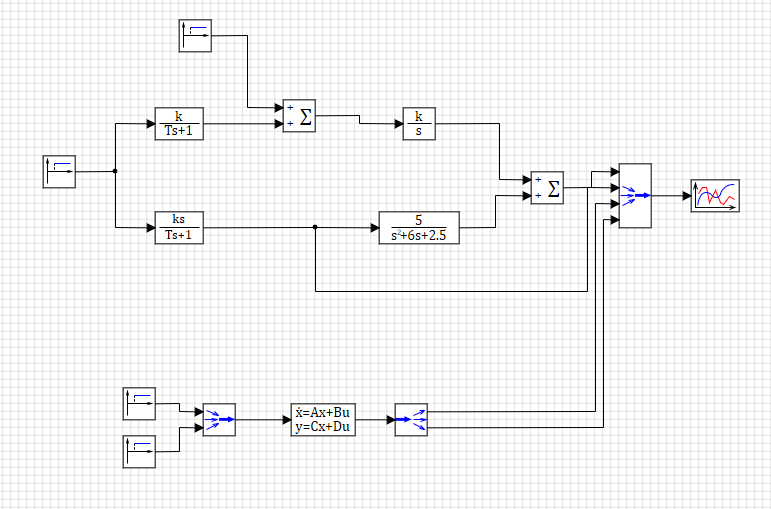
\includegraphics[width=.7\textwidth]{png/scheme1.png}
		\caption{Схема для моделирования многосвязной системы}
		\label{scheme1}
	\end{figure}
	
	В соответствии с полученными в подготовке выражениями (\ref{matrices1}) матрицы системы в переменных состояния принимают вид:
	\begin{equation*}
		A = \begin{bmatrix}
			-10 & 0 & 0 & 0 & 0 \\
			1,1 & 0 & 0 & 0 & 0 \\
			0 & 0 & -2,5 & 0 & 0 \\
			0 & 0 & 0 & 0 & 1 \\
			0 & 0 & 5 & -2,5 & -6
		\end{bmatrix},\;
		B = \begin{bmatrix}
			20 & 0 \\
			0 & 1,1 \\
			-24,375 & 0 \\
			0 & 0 \\
			48,75 & 0		
		\end{bmatrix},\;
	\end{equation*}
	\begin{equation*}
		C = \begin{bmatrix}
			0 & 1 & 0 & 1 & 0 \\
			0 & 0 & 1 & 0 & 0
		\end{bmatrix},\;
		D = \begin{bmatrix}
			0 & 0 \\
			9,75 & 0
		\end{bmatrix}
	\end{equation*}

	В блоке переменных состояния в среде \textit{SimInTech} все эти матрицы указываются в транспонированном виде. В результате моделирования переходные процессы, представленные на рис. \ref{graph1}. Видим, что графики для обоих реализации многосвязной системы совпали, значит они являются эквивалентными и ошибок при переходе от одного представления к другому допущено не было.
	
	\begin{figure}[h]
		\centering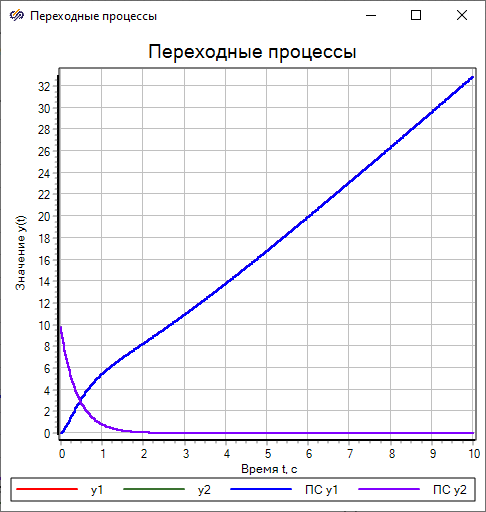
\includegraphics[width=.45\textwidth]{png/graph1.png}
		\caption{Переходные процессы, полученные в результате моделирования многосвязной системы}
		\label{graph1}
	\end{figure}
	
	\subsection{Моделирование замкнутой системы}
	
	Для моделирования была собрана схема, представленная на рис. \ref{scheme2}. Так же как и при моделировании многосвязной системы система собрана в двух представлениях.
		
	\begin{figure}[h]
		\centering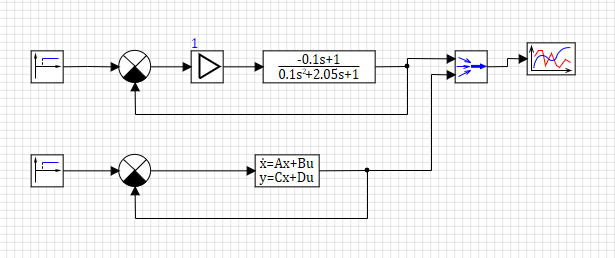
\includegraphics[width=.6\textwidth]{png/scheme2.png}
		\caption{Схема для моделирования замкнутой системы}
		\label{scheme2}
	\end{figure}

	Матрицы системы в переменных состояния в соответствии с выражениями, полученными в подготовке (\ref{matrices2}):
		\begin{equation*}
		A = \begin{bmatrix}
			-20 & 0 \\
			0 & -0,5
		\end{bmatrix},\; 
		B = \begin{bmatrix}
			-1,54 \\ 0,54
		\end{bmatrix},\;
		C = \begin{bmatrix}
			1 & 1
		\end{bmatrix},\;D=0
	\end{equation*}

	Здесь $k_\text{р}$ положен равным 1. В результате моделирования, получили процессы, представленные на рис. \ref{graph2}. Как видим, процессы в обоих представлениях системы совпали, значит они являются эквивалентными.
	
	\begin{figure}[h]
		\centering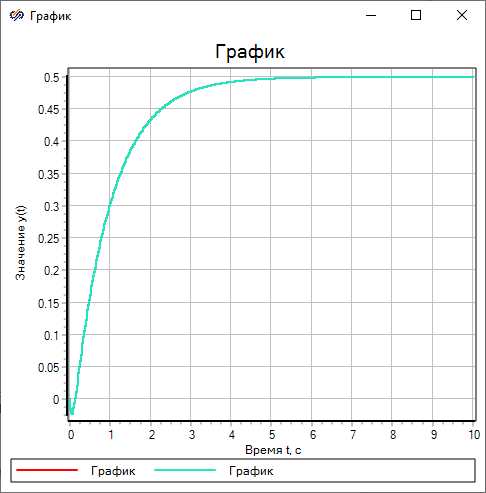
\includegraphics[width=.45\textwidth]{png/graph2.png}
		\caption{Переходные процессы, полученные в результате моделирования замкнутой системы}
		\label{graph2}
	\end{figure}

	\textbf{Устойчивость}. В соответствии с выражением (\ref{kpr}), полученным в подготовке имеем $k_\text{пр} = 20,5$. Проверяем экспериментально, и получаем, что при $k_\text{р} = 20,5$ действительно процессы в системе являются незатухающими: рис. \ref{graph4}.
	
	\begin{figure}[h]
		\centering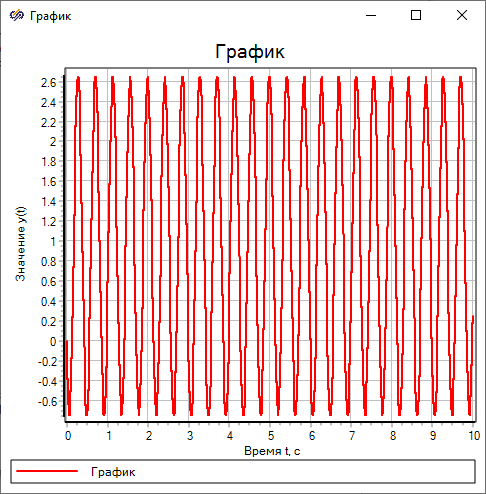
\includegraphics[width=.45\textwidth]{png/graph4.png}
		\caption{Процессы в замкнутой системе при $k_\text{р} = 20,5$}
		\label{graph4}
	\end{figure}

	Исследуем экспериментально влияние параметра $\tau = \dfrac{T_2}{T_1}$ на значение $k_\text{пр}$. Полученные значения занесены в табл. \ref{table} и построены на графике, представленном на рис. \ref{krp(tau)}. Как видно по графику, полученная зависимость совпадает с выведенной в подготовке (\ref{kpr}) и является линейной.

	\noindent\begin{minipage}{.5\textwidth}
		\begin{center}
			\begin{tabular}{|c|c|}
				\hline
				$\tau = \frac{T_2}{T_1}$ & $k_\text{пр}$ \\[0.3em] \hline
				10                       & 10,5          \\ \hline
				20                       & 20,5          \\ \hline
				40                       & 40,5          \\ \hline
				60                       & 60,5          \\ \hline
				100                      & 100,5         \\ \hline
			\end{tabular}
		\end{center}
		\captionof{table}{Полученная зависимость $k_\text{пр}(\tau)$}
		\label{table}	
	\end{minipage}
	\begin{minipage}{.5\textwidth}
		\begin{filecontents*}{data2.csv}
			a,b
			20,20.5
			40,40.5
			10,10.5
			100,100.5
			60,60.5
		\end{filecontents*}
		
		\begin{center}
			\begin{tikzpicture}
				\begin{axis}[
					xlabel={$\tau=\frac{T_2}{T_1}$},
					ylabel={$k_\text{пр}$},
					xlabel style={above right},
					xmin=0, xmax = 115,
					ylabel style = {above right},
					ymin=0, ymax = 115,
					axis lines = center,
					]
					\addplot[mark=*] table [x=a, y=b, col sep=comma] {data2.csv};
					\node [below right] at (0,0) {0};
				\end{axis}
			\end{tikzpicture}
			\captionof{figure}{График зависимости $k_\text{пр}(\tau)$}
			\label{krp(tau)}	
		\end{center}
	\end{minipage}

	\subsection{Блоки для исследования систем}
	
	Рассмотрим применение готовых блоков из \textit{SimInTech} для исследования частотных и алгебраических характеристик систем. Собрана схема, представленная на рис. \ref{scheme3}.
	
	\begin{figure}[h]
		\centering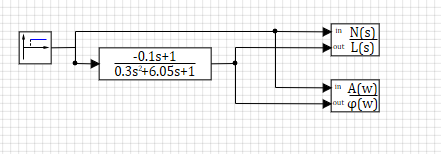
\includegraphics[width=.7\textwidth]{png/scheme3.png}
		\caption{Схема для исследования характеристик системы}
		\label{scheme3}
	\end{figure}

	В результате моделирования такой схемы мы можем увидеть годограф Найквиста, нули, полюсы системы и другие характеристики: рис. \ref{graph5}-\ref{info}.
	
	\noindent\begin{minipage}{.4\textwidth}
		\centering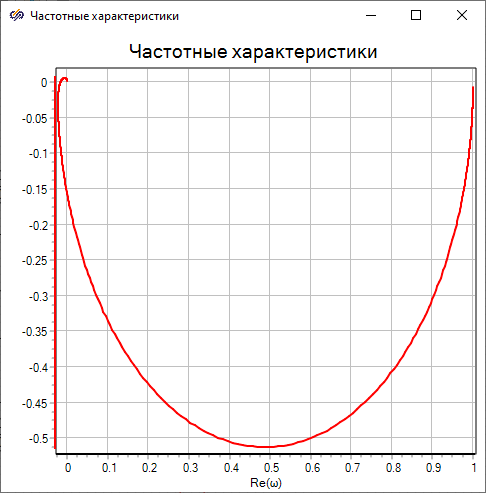
\includegraphics[width=.8\textwidth]{png/graph5.png}
		\captionof{figure}{Годограф Найквиста системы}
		\label{graph5}
	\end{minipage}
	\begin{minipage}{.6\textwidth}
		\centering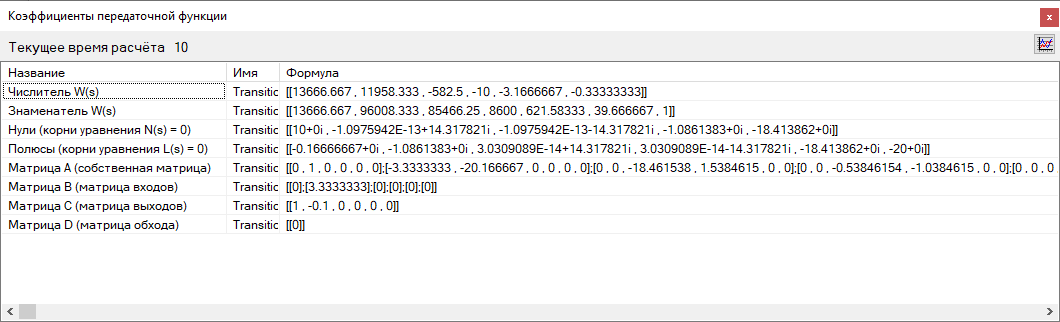
\includegraphics[width=\textwidth]{png/info.png}
		\captionof{figure}{Алгебраические характеристики системы}
		\label{info}
	\end{minipage}
	
	\section{Выводы}
	
	В этой работе было проведено моделирование двух систем: многосвязной и замкнутой. Для этого системы были представлены в переменных состояния. На практике при работе в \textit{SimInTech} задание системы в типовых звеньях и переменных состояния давало одинаковые результаты. 
	
	Для замкнутой системы была исследована устойчивость и зависимость предельного коэффициента усиления от параметра, характеризуемого постоянными времени системы, $k_\text{пр}\left(\frac{T_2}{T_1}\right)$. Полученные результаты совпали с теми, что были получены в подготовке к работе.
	
	Была исследована возможность использования типовых блоков \textit{SimInTech} для получения частотных и алгебраических характеристик системы.
	
\end{document}
